\documentclass[8pt]{article}

\usepackage{fullpage}
\usepackage{tikz}
\usepackage{xcolor}
\usepackage{graphicx}
\usepackage{float}
\usepackage{wrapfig}
\usepackage{titlesec}
\setcounter{secnumdepth}{4}
\graphicspath{ {./pictures/} }
\usepackage[a4paper,bindingoffset=0.2in,%
            left=0.5in,right=0.5in,top=1in,bottom=1in,%
            footskip=.25in]{geometry}
\usetikzlibrary{shapes.geometric, arrows}
\tikzstyle{startstop} = [rectangle, rounded corners, minimum height=0.5cm,text centered, draw=black, fill=red!30]
\tikzstyle{io} = [trapezium, trapezium left angle=70, trapezium right angle=110, minimum height=0.8cm, text centered, draw=black, fill=blue!30]
\tikzstyle{process} = [rectangle, minimum width=1cm, minimum height=1cm, text centered, draw=black, fill=orange!30]
\tikzstyle{decision} = [diamond, minimum width=1cm, minimum height=1cm, text centered, draw=black, fill=green!30]
\tikzstyle{arrow} = [thick,->,>=stealth]
\tikzstyle{line} = [thick,-,>=stealth]

\begin{document}

\title{ARM Final Report}
\author{Fawwaz Abdullah (ffa20), Robert Buxton (rb419), \\Edward Hartley (ech120), Wojtek Sowinski (ws420) }

\maketitle

\section{Assembler implementation}

\subsection{Data Structures}

\begin{itemize}

    \item \textbf{Map} (\texttt{StringUintMap}) A map implemented using a
    red-black tree and hashing function to allow strings to be mapped to unsigned
    32 bit integers. This is used in two cases. Firstly to map branch tags to
    memory locations and secondly to translate assembly inputs to their respective
    enum representations to be parsed. The root (a MapNode) and number of nodes is stored.

    \item \textbf{Tree Node} (\texttt{MapNode}) A node in the red-black tree that
    stores the hash identifier of the node, the number of symbols with this hash,
    a list of symbols (\_\_StringUintPair\_\_), the colour of the node which is used for balancing, the
    parent node, and the left and right children.

    \item \textbf{Symbol Pair} (\texttt{\_\_StringUintPair\_\_}) A struct holding a
    string (identifier of the symbol) and a corresponding value (either an
    address or enum value).

    \item \textbf{Query Result} (\texttt{QueryResult}) A struct returned when searching the map;
    it holds a Boolean describing whether a result was found and has a field for storing that result.

\end{itemize}

\begin{minipage}{0.45\textwidth}
\subsection{Program Structure}

\begin{itemize}
    \item \texttt{parser.c} \\Collects the symbols in the first pass of the
    input data and resets the file to be reread for the second pass.
    \item \texttt{symbols.c} \\Contains the functions that create and interact with the
    symbol map used to map labels to memory addresses.
    \item \texttt{assemble.c} \\Initalises the maps used in the assembler. Then
    passes over the file twice mapping labels to memory addresses and converting
    instructions into binary.
    \item \texttt{branch.c} \\Handles converting the branch instruction.
    \item \texttt{dataprocessing.c} \\Handles converting the data processing
    instructions.
    \item \texttt{multiply.c} \\Handles the multiply instructions.
    \item \texttt{singledatatransfer.c} \\Handles the single data transfer instructions.
\end{itemize}
\end{minipage}%
\hfill
\begin{minipage}{0.45\textwidth}

\begin{figure}[H]
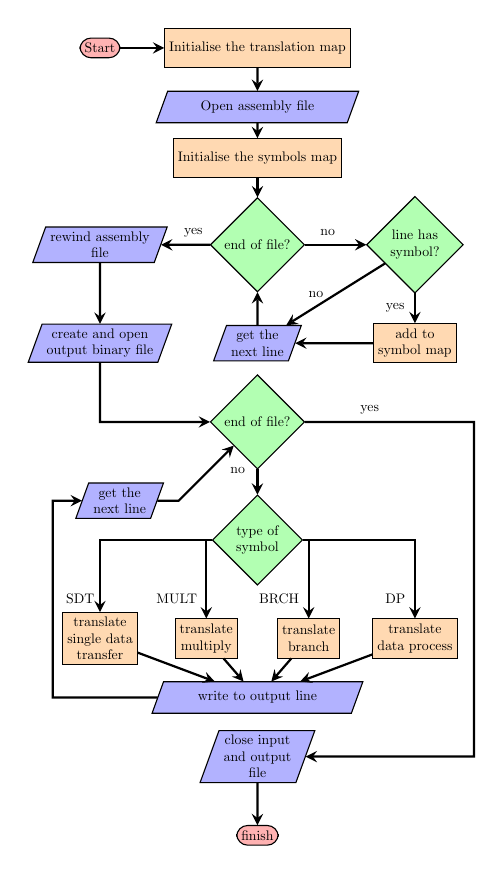
\begin{tikzpicture}[node distance=2cm]
    \node (start) [scale=0.5, startstop, align=center] at (0,0) {Start};
    \node (init_map) [scale=0.5, process, align=center] at (2,0) {Initialise the translation map};
    \node (open_file) [scale=0.5, io, align=center] at (2,-0.75) {Open assembly file};
    \node (init_map2) [scale=0.5, process, align=center] at (2,-1.4) {Initialise the symbols map};
    \node (end_file?) [scale=0.5, decision, align=center] at (2,-2.5) {end of file?};
    \node (is_symbol) [scale=0.5, decision, align=center] at (4,-2.5) {line has \\ symbol?};
    \node (add_map) [scale=0.5, process, align=center] at (4,-3.75) {add to \\ symbol map};
    \node (get_line) [scale=0.5, io, align=center] at (2,-3.75) {get the \\ next line};
    \node (rewind) [scale=0.5, io, align=center] at (0,-2.5) {rewind assembly \\ file};
    \node (create_file) [scale=0.5, io, align=center] at (0,-3.75) {create and open \\ output binary file};
    \node (end_file?2) [scale=0.5, decision, align=center] at (2,-4.75) {end of file?};
    \node (symbol_type) [scale=0.5, decision, align=center] at (2,-6.25) {type of \\ symbol};
    \node (sdt) [scale=0.5, align=center, process] at (0,-7.5) {translate \\ single data \\ transfer };
    \node (mult) [scale=0.5, align=center, process] at (1.35,-7.5) {translate \\ multiply};
    \node (brch) [scale=0.5, align=center, process] at (2.65,-7.5) {translate \\ branch};
    \node (dp) [scale=0.5, align=center, process] at (4,-7.5) {translate \\ data process};
    \node (write_out) [scale=0.5, io, align=center] at (2,-8.25) {write to output line};
    \node (get_line2) [scale=0.5, io, align=center] at (0.25,-5.75) {get the \\ next line};
    \node (close) [scale=0.5, io, align=center] at (2,-9) {close input \\ and output \\file};
    \node (finish) [scale=0.5, startstop, align=center] at (2,-10) {finish};

    \draw [arrow] (start) -- (init_map);
    \draw [arrow] (init_map) -- (open_file);
    \draw [arrow] (open_file) -- (init_map2);
    \draw [arrow] (init_map2) -- (end_file?);
    \draw [arrow] (end_file?) -- node[scale=0.5, xshift = 0.2cm, yshift=0.3cm] {yes} (rewind);
    \draw [arrow] (end_file?) -- node[scale=0.5, xshift = -0.2cm, yshift=0.3cm] {no} (is_symbol);
    \draw [arrow] (is_symbol) -- node[scale=0.5, xshift = -0.5cm] {yes} (add_map);
    \draw [arrow] (is_symbol) -- node[scale=0.5, xshift = -0.5cm] {no} (get_line);
    \draw [arrow] (add_map) -- (get_line);
    \draw [arrow] (get_line) -- (end_file?);
    \draw [arrow] (rewind) -- (create_file);
    \draw [arrow] (create_file) -- (0,-4.75) -- (end_file?2);
    \draw [arrow] (end_file?2) -- node[scale=0.5, xshift = -0.5cm, yshift=0.3cm] {no} (symbol_type);
    \draw [arrow] (symbol_type) -| node[scale=0.5, yshift = -1.5cm, xshift = -0.5cm] {SDT} (sdt);
    \draw [arrow] (symbol_type) -| node[scale=0.5, yshift = -1.5cm, xshift = -0.75cm] {MULT} (mult);
    \draw [arrow] (symbol_type) -| node[scale=0.5, yshift = -1.5cm, xshift = -0.75cm] {BRCH} (brch);
    \draw [arrow] (symbol_type) -| node[scale=0.5, yshift = -1.5cm, xshift = -0.5cm] {DP} (dp);
    \draw [arrow] (sdt) -- (write_out);
    \draw [arrow] (mult) -- (write_out);
    \draw [arrow] (brch) -- (write_out);
    \draw [arrow] (dp) -- (write_out);
    \draw [arrow] (write_out) -- (-0.6,-8.25) -- (-0.6,-5.75) -- (get_line2);
    \draw [arrow] (get_line2) -- (1,-5.75) -- (end_file?2);
    \draw [arrow] (end_file?2) -- node[scale=0.5, xshift = -0.5cm, yshift=0.3cm] {yes}
     (4.75,-4.75) -- (4.75,-9) -- (close);
    \draw [arrow] (close) -- (finish);
\end{tikzpicture}
\caption{A flowchart demonstrating program flow in assembler.c.}
\end{figure}
\end{minipage}

\section{Extension: Rubik's Cube solver}
\subsection{Description}
Our group chose to build a Rubik's cube solving machine as our extension. The machine
needed to be able to scramble and solve a 3 $\times$ 3 Rubik's cube. To complete this project, we split the team
in two sections with Robert working on the physical side, designing
and building the machine, while Fawwaz, Edward and Wojtek worked on the algorithm behind
solving the cube.

\subsection{The Machine}

\subsubsection{Design}

We decided to build the robot using primarily VEX Robotics parts we already had which helped
reduce the cost of the robot significantly. The machine was controlled by an ARM Cortex-A9 processor and
used 6 motors with built-in encoders to rotate and track the positions of the 6 faces of the 
Rubik's cube. The program took a scrambled Rubik's cube and solved it by rotating its faces according to our solver's output. 

\begin{minipage}{0.45\textwidth}
\begin{figure}[H]
\centering
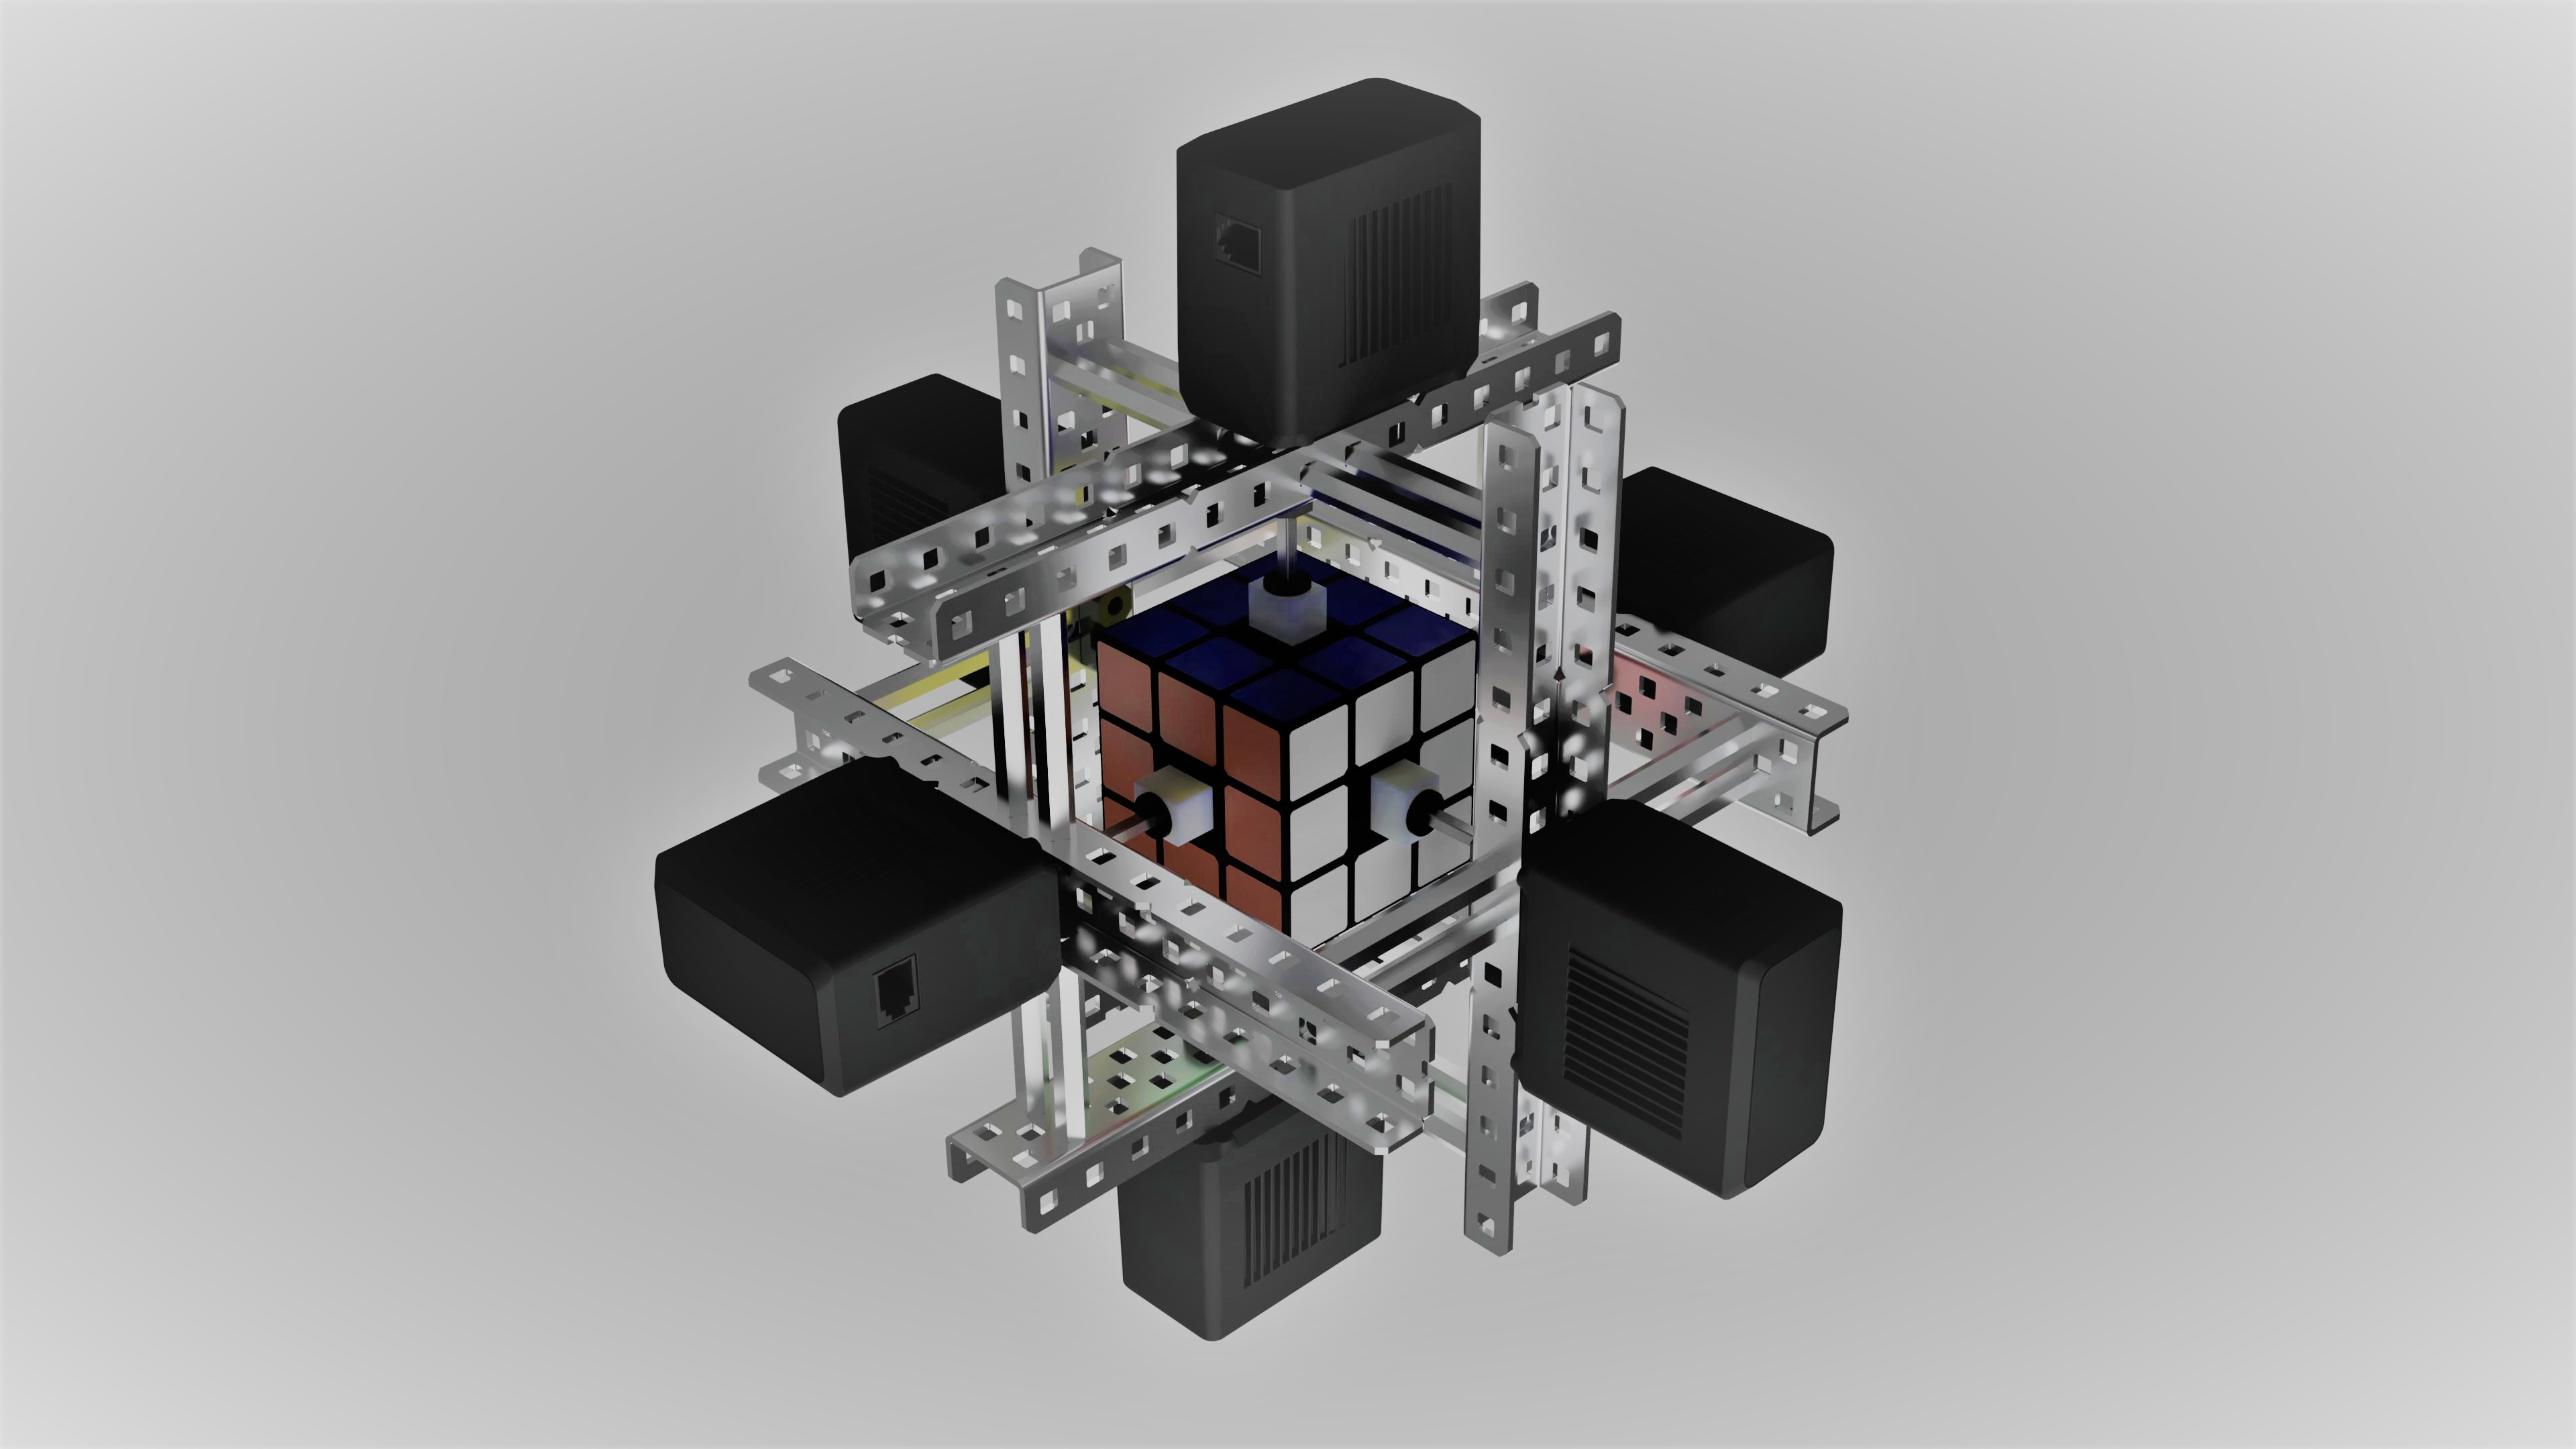
\includegraphics[scale=0.05]{main cad.jpg}
\caption{A CAD rendering of the machine created in Autodesk Fusion 360 created
before building the robot.}
\end{figure}
\end{minipage}%
\hfill
\begin{minipage}{0.45\textwidth}
\begin{figure}[H]
\centering
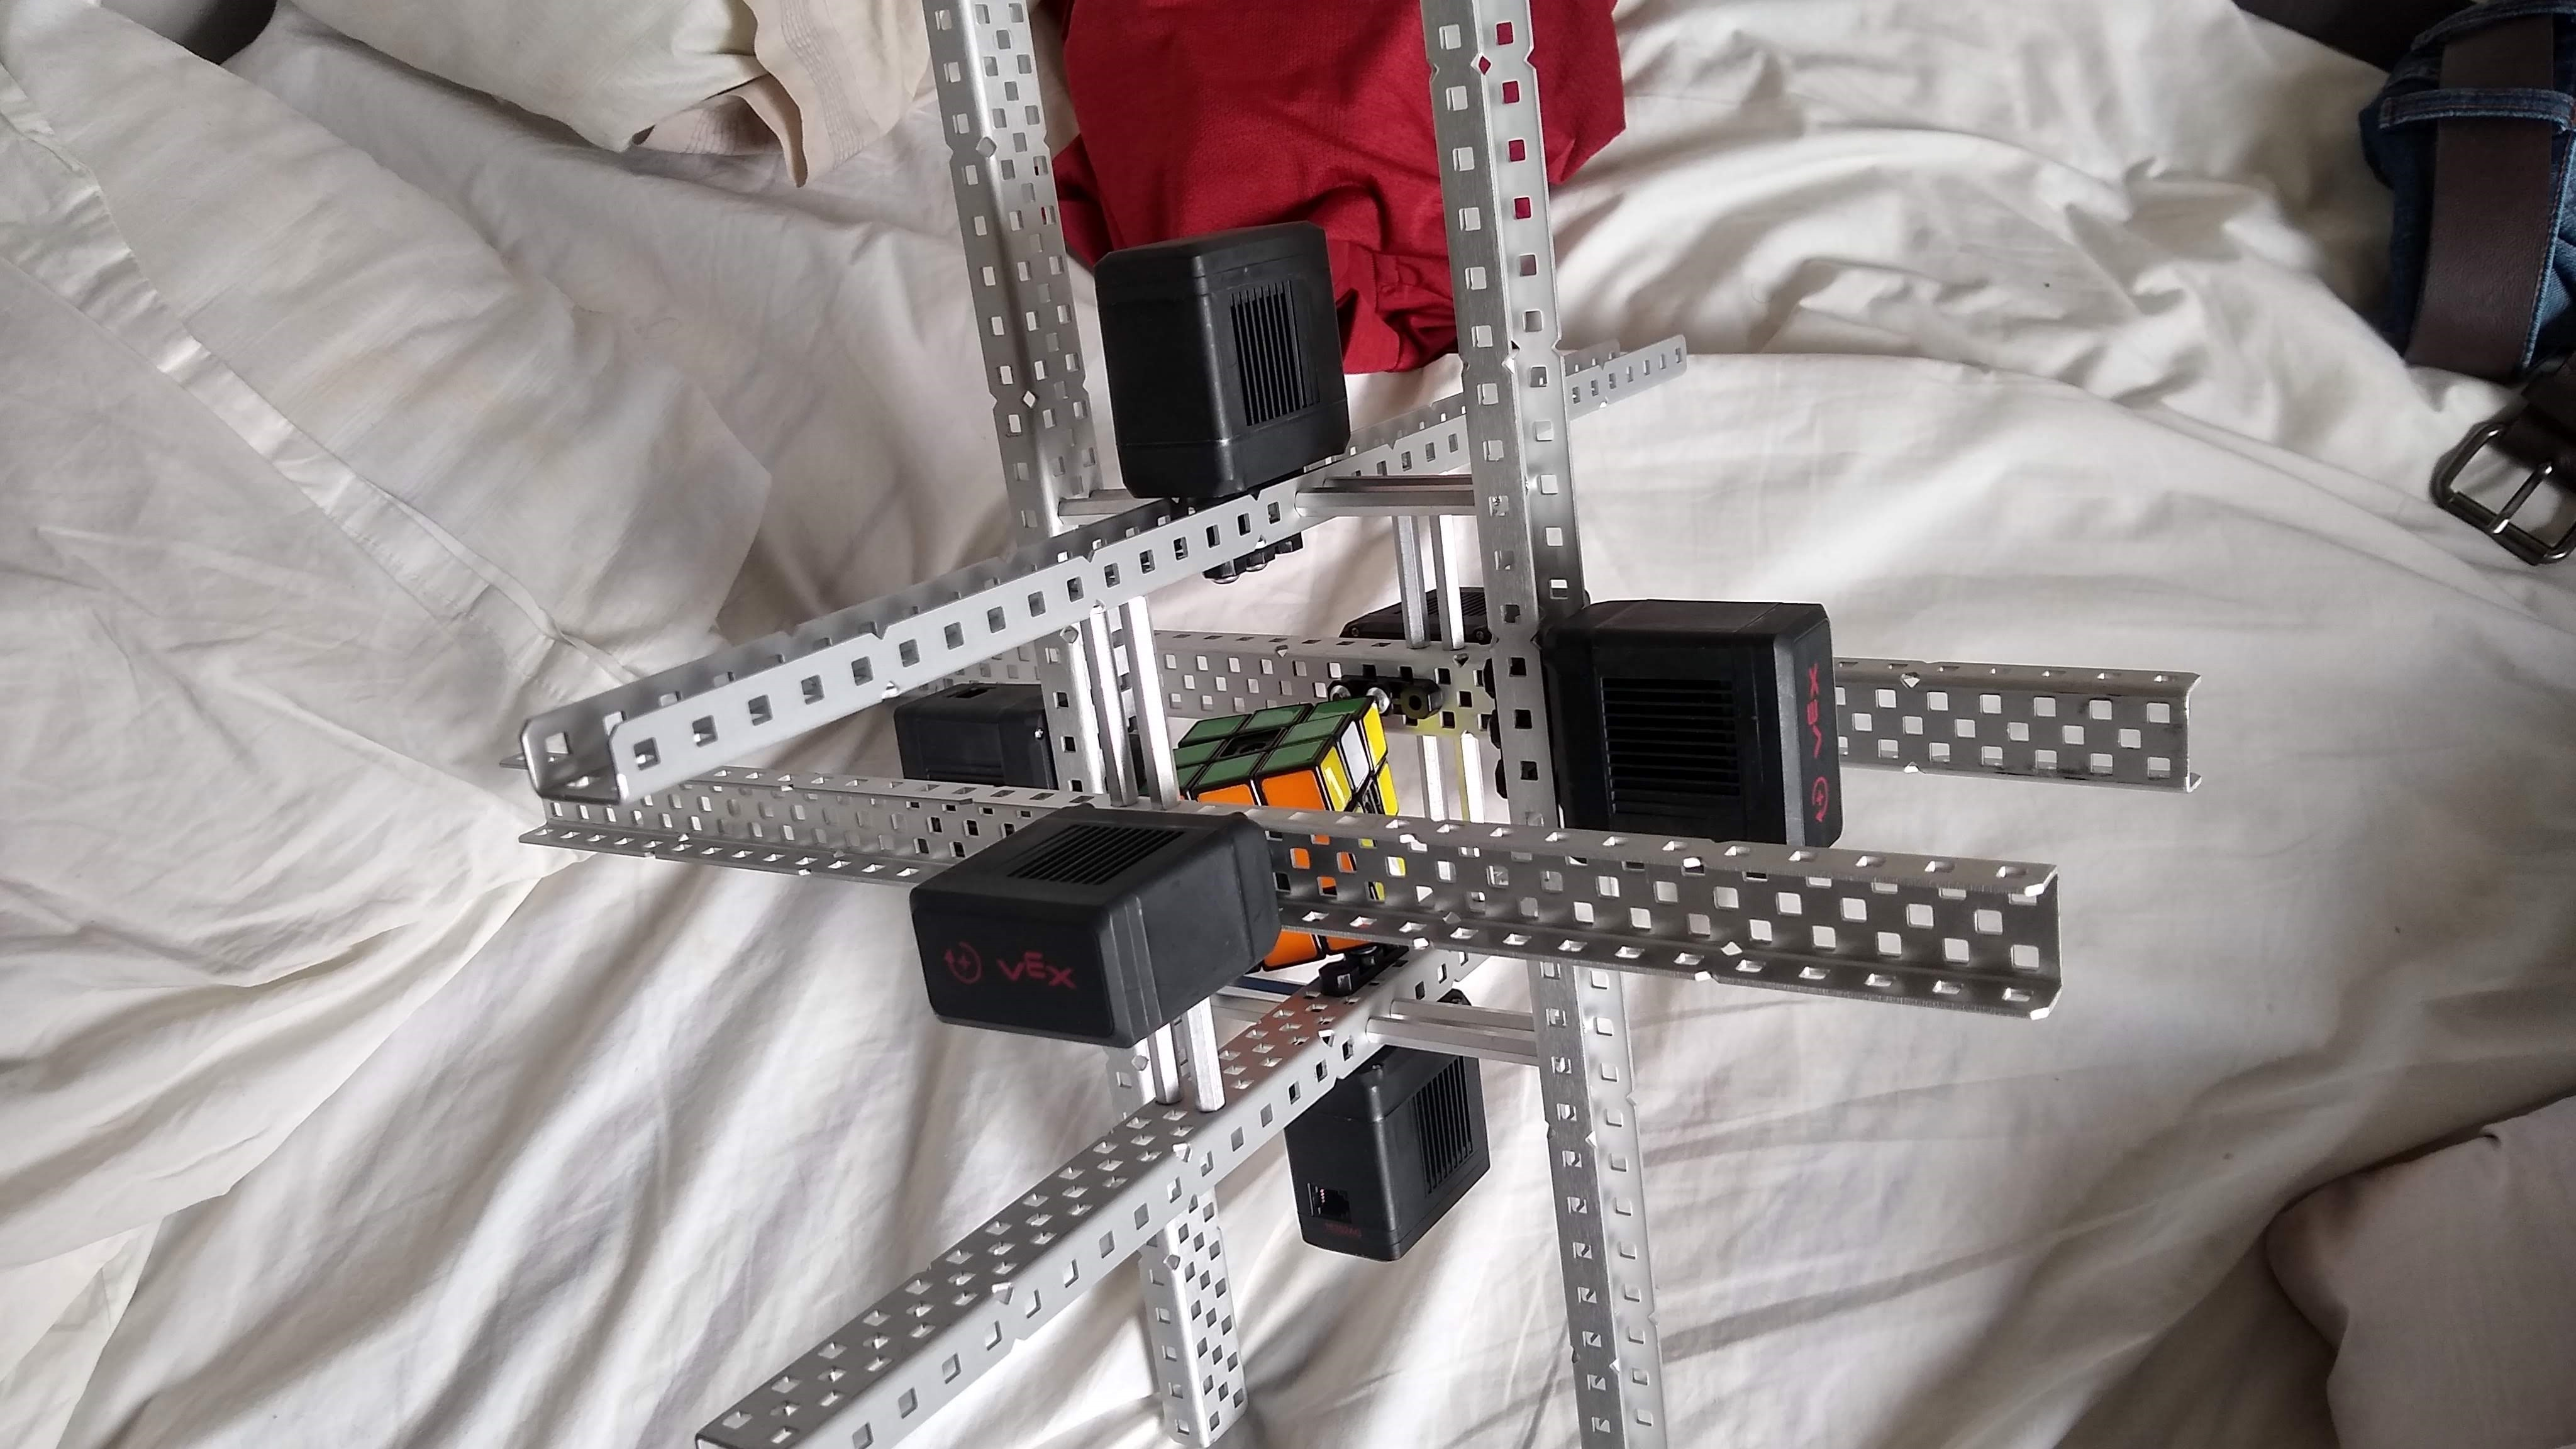
\includegraphics[scale=0.11]{final machine.jpg}
\caption{The final finished machine}
\end{figure}
\end{minipage}

\subsubsection{Building process}

Firstly we designed the machine in CAD using Autodesk Fusion 360. We decided it should 
consist of a simple frame of aluminum to which we would attach the 6 motors at perpendicular 
angles. We used an UP mini 2 3D printer at the White City Campus advanced hackspace to create 
custom parts to connect the axels and Rubik's cube centre pieces to allow the face to be rotated 
by a motor. It was important that these pieces were strong as they would would undergo 
high stress. We then put the machine together and started testing it.

\subsubsection{Challenges}

The main problem we came across was that when rotating faces there could be an 
up to 20 degree error in the final position. This was because a standard rubik's
 cube is quite loose and this results in quite a bit of give between the centre 
 pieces and the surrounding ones. This meant that even if we rotated the centre 
 perfectly we could not guarantee the rest of face was in the correct place. If 
 a face was not within a certain position when attempting to rotate, the whole 
 machine would seize up and we would have to manually reset it. This meant that
  we could not reliably physically solve a cube with solutions longer than about 6 moves.


\subsubsection{Future improvements}

If we were to keep working on this project the first thing we would need to fix 
would be the face alignment issue. This could be done relatively easy by replacing
our current Rubik's cube with one that has magnets inside to assist with the alignment.
It is a shame we didn't know these existed before we started the project. Currently 
the machine is also quite unstable and we could definitely be rebuilt to be more sturdy. 
It would also be interesting to add a camera to the machine to detect the current cube state
automatically rather than having to rely on manual user input.


\subsection{The solving algorithm}
\subsubsection{Data Structures}

\begin{itemize}

    \item \textbf{Cube Movement} (\texttt{Movement}) A struct holding the face to
    be moved and the direction to be moved (clockwise, anti-clockwise or double).

    \item \textbf{Cube State} (\texttt{CubeState}) Holds the current state of the
    faces of the cube as six two-dimensional arrays of Colours (an enum). It also contains
    a history of all movements that have been applied to the cube and how many moves
    are in that list.

    \item \textbf{Unfolding Template} (\texttt{UnfoldTemplate}) These precomputed
    structures hold information describing how each face connects to its neighbouring
    edges with regards to their array represeantation. When a face of the cube is rotated, this
    information is used to rotate the neighbouring edges along with it.

\end{itemize}

\subsubsection{Program structure}

\begin{minipage}{0.45\textwidth}
    \begin{itemize}
        \item \texttt{solver.c} \\ Initialises the priority queue and hash tree then
        evaluates and expands states from the priority queue until either there are no states
        left in the queue or a solution has been found. This is an
        implementation of an A* graph search.
        \item \texttt{cubestate.c} \\ Holds all the functions used to modify and interact
        with cube states.
        \item \texttt{hashtree.c}\\  Contains an implementation for the red black tree we
        use for storing which cube state hashes we have visited.
        \item \texttt{movequeue.c}\\ Contains an implementation for the priority queue we use
        for deciding the next state to visit.
        \item \texttt{ida\_star.c (unused)}\\ An alternative implementation
        of the solver using an IDA* graph search (unfinished due to time constraints).
        \item \texttt{testcubestate.c}\\ Tests to make sure cube state functions
        work as intended.
        \item \texttt{testmovequeue.c}\\ Tests to make sure the move priority queue
        functions correctly.
        \item \texttt{testsolver.c}\\ Tests to make sure the whole program is working as
        intended. Also used to measure progress in solving ability.
        \item \texttt{estimate\_cost}\\ Estimates the cost of a solution through a particular
        state by summing the weight of the path from the start to there, and any one of a few heuristic functions
        we were experimenting with.


    \end{itemize}
    \end{minipage}%
    \hfill
    \begin{minipage}{0.45\textwidth}

    \begin{figure}[H]
    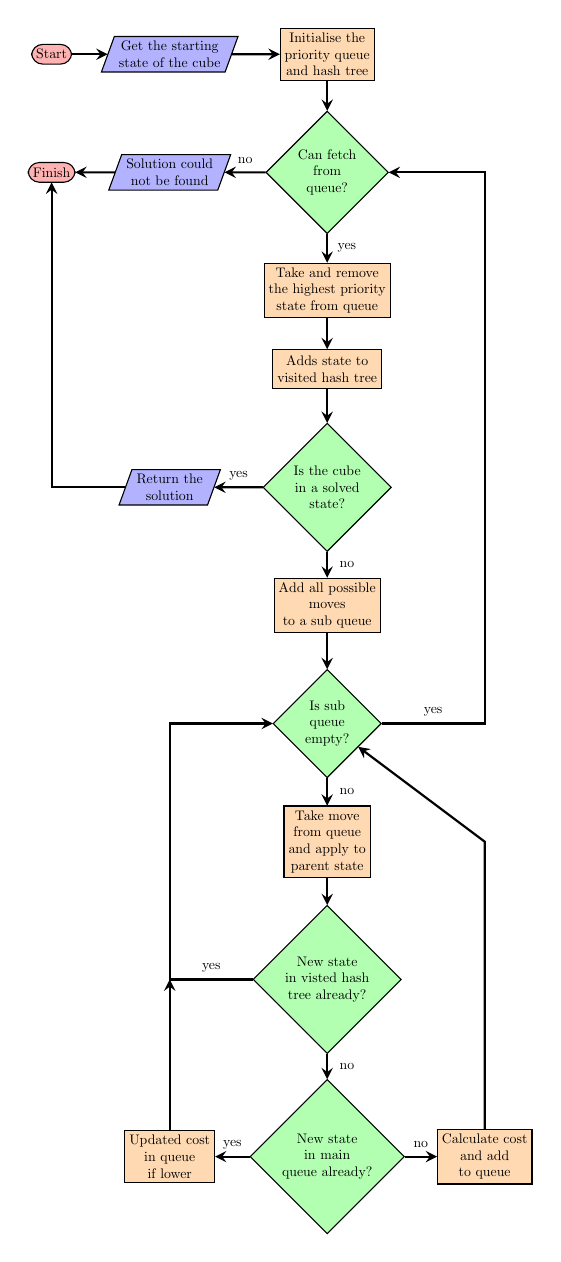
\begin{tikzpicture}[node distance=2cm]
        \node (start) [scale=0.5, startstop, align=center] at (0,0) {Start};
        \node (starting_state) [scale=0.5, io, align=center] at (1.5,0) {Get the
        starting \\ state of the cube};
        \node (init_main) [scale=0.5, process, align=center] at (3.5,0) {Initialise the\\
        priority queue \\ and hash tree};
        \node (check_empty) [scale=0.5, decision, align=center] at (3.5,-1.5)
        {Can fetch \\ from \\ queue?};
        \node (not_solved) [scale=0.5, io, align=center] at (1.5,-1.5)
        {Solution could \\ not be found};
        \node (finish) [scale=0.5, startstop, align=center] at (0,-1.5) {Finish};
        \node (pop) [scale=0.5, process, align=center] at (3.5,-3) {Take and remove
        \\ the highest priority \\ state from queue};
        \node (add_hash) [scale=0.5, process, align=center] at (3.5,-4)
        {Adds state to \\ visited hash tree};
        \node (check_solved) [scale=0.5, decision, align=center] at (3.5,-5.5)
        {Is the cube \\ in a solved \\ state?};
        \node (solved) [scale=0.5, io, align=center] at (1.5, -5.5)
        {Return the \\ solution};
        \node (expand_move) [scale=0.5, process, align=center] at (3.5,-7)
        {Add all possible \\ moves\\ to a sub queue };
        \node (sub_queue_empty?) [scale=0.5, decision, align=center] at (3.5,-8.5)
        {Is sub \\ queue  \\ empty?};
        \node (take_move) [scale=0.5, process, align=center] at (3.5,-10)
        {Take move \\ from queue \\ and apply to \\ parent state};
        \node (move_in_queue?) [scale=0.5, decision, align=center] at (3.5,-11.75)
        {New state \\in visted hash \\ tree already?};
        \node (in_main_queue?) [scale=0.5, decision, align=center] at (3.5,-14)
        {New state \\ in main\\ queue already?};
        \node (update_cost) [scale=0.5, process, align=center] at (1.5,-14)
        {Updated cost \\ in queue \\ if lower};
        \node (add_to_queue) [scale=0.5, process, align=center] at (5.5,-14)
        {Calculate cost \\and add \\ to queue};



        \draw [arrow] (start) -- (starting_state);
        \draw [arrow] (starting_state) -- (init_main);
        \draw [arrow] (init_main) -- (check_empty);
        \draw [arrow] (check_empty) -- node[scale=0.5, yshift=0.3cm] {no} (not_solved);
        \draw [arrow] (not_solved) -- (finish);
        \draw [arrow] (check_empty) -- node[scale=0.5, xshift=0.5cm] {yes} (pop);
        \draw [arrow] (pop) -- (add_hash);
        \draw [arrow] (add_hash) -- (check_solved);
        \draw [arrow] (check_solved) -- node[scale=0.5, yshift=0.3cm] {yes} (solved);
        \draw [arrow] (solved) -| (finish);
        \draw [arrow] (check_solved) -- node[scale=0.5, xshift=0.5cm] {no} (expand_move);
        \draw [arrow] (expand_move) -- (sub_queue_empty?);
        \draw [arrow] (sub_queue_empty?) -- node[scale=0.5, yshift=0.3cm] {yes} (5.5,-8.5) -- (5.5,-1.5) -- (check_empty);
        \draw [arrow] (sub_queue_empty?) -- node[scale=0.5, xshift=0.5cm] {no} (take_move);
        \draw [arrow] (take_move) -- (move_in_queue?);
        \draw [arrow] (move_in_queue?) -- node[scale=0.5, yshift=0.3cm] {yes} (1.5,-11.75) -- (1.5,-8.5) -- (sub_queue_empty?);
        \draw [arrow] (move_in_queue?) -- node[scale=0.5, xshift=0.5cm] {no} (in_main_queue?);
        \draw [arrow] (in_main_queue?) -- node[scale=0.5, yshift=0.3cm] {yes} (update_cost);
        \draw [arrow] (update_cost) -- (1.5,-11.75);
        \draw [arrow] (in_main_queue?) -- node[scale=0.5, yshift=0.3cm] {no} (add_to_queue);
        \draw [arrow] (add_to_queue) -- (5.5,-10) -- (sub_queue_empty?);

    \end{tikzpicture}
    \caption{A flowchart demonstrating program flow in solver.c.}
    \end{figure}
\end{minipage}

\subsubsection{Challenges and Alternative Algorithms}

Our Rubik's cube solver uses the A* path finding algorithm to find the shortest path
from the cube's inintial state to a solved cube. When we first implemented this,
the algorithm's memory usage and speed both presented major challenges.

Due to the way we have used a priority queue in order to track incoming cube states,
and every move exponentially increases the number of potential next cube states, the
program consumed 4 GB of heap space faster than it can even solve some basic cubes.
This was a problem, as our intended motor controller only had around 128 MB of total RAM.

One way we remedied this issue is by testing a variety of heuristics in an attempt to
increase the likelihood of the A* algorithm finding the solution early. We also attempted
the following alternative algorithms:
\begin{itemize}
    \item \texttt{Kociemba's algorithm} \\ This algorithm created by Herbert Kociemba
    has two phases. In the first phase, a searching algorithm (such as A*)
    is used to find a path from the initial state to a subset of states referred to as G1.
    This subset is characterised by the fact that, once a cube is in G1, a solution can
    be obtained using only 10 different moves as opposed to the usual 18. This speeds up
    the second phase which is finding a path from G1 to a solved state.
    \item \texttt{Iterative Deepening A* (IDA*)} \\ This is a variant of the A* algorithm
    which uses a stack instead of a queue. It starts with an expected upper bound on
    the length of the solution, searches for solutions of length up to that bound in a
    depth-first fashion and, if no solution is found, the upper bound is increased.
    Many paths are explored multiple times which makes the algorithm slower but the use
    of a stack and the depth-first nature of the search makes it more memory efficient than A*.
\end{itemize}

The use of Kociemba's algorithm allowed us to solve more scrambled cubes more reliably but
it also resulted in solutions which took more moves than necessary. Due to time constraints,
we weren't able to fully implement IDA*. Were we able to do that, the next step would have been
to combine IDA* with Kociemba's two-phase approach.

Another way we partially remedied the issue was to go through and shrink down as many of the structs as possible
while still being able to store all the necessary data.
For example, the cube state field that held the colour data was shortened to use an array of unsigned
8-bit values instead of the default enum size, and how the movement structure used bit fields to squeeze
the fields that define what face its rotating (and in what direction) into a single 8-bit value.
By doing this, we extended the number of items that can be held inside the queue before it overflowed.

One avenue we didn't explore was to rewrite the hash tree as an array instead of a discrete tree structure.
This would have reduced the number of fields inside a single tree node, which would have reduced the tree's overall size.
Another way we didn't consider was to use a smaller integer as a hash. That has an issue, as the number of possible cube states
is about four times as many as there are 64-bit integers. Therefore using something like a 32-bit integer would have exponentially
increased the possible errors generated by hash collisions (as our queue insertion depended on a tree to prevent duplicates, and to
allow an O(log n) update key operation instead of an O(n) operation).

\subsection{Testing and Debugging}

\subsubsection{Test Suite}

All testing for this extension was handled using a unit testing library (created ourselves, found in \texttt{[root]/extension/testsuite}).

The code was tested in parts, with behaviour mimicking the behavior of such unit testing libraries as \texttt{JUnit}, where a test file comprises of tester functions (a \texttt{void} function that takes no parameters), and an array of tagged function pointers to those functions to give friendly names in the output log for each test function.

The main function in a test file effectively iterates through all the tagged functions and runs them.
If a test function fails (i.e. an ``assertion" fails), the test function terminates and the next test function is executed.
A \texttt{setjmp} / \texttt{longjmp} pair was used to provide this functionality, in order to avoid using C's default \texttt{assert} function.

This easily modifiable, modular testing suite meant any member of the team could add a test to check that the code they created worked.
We had a range of tests that covered different scopes of functions so that problems could be diagnosed by looking at exactly which tests passed and failed.
Finally, while for completed code much of the testsuite was automated and used to ensure previous code remained valid, we also found functions such as 
\texttt{print\_cubestate} useful during production (e.g. when programming the application of rotations to a cube).

\subsubsection{Debugging}

GDB was used in order to help track down infinite loops and errant logic errors in our code, and Valgrind was used to help point out where memory was leaking, as the program deals with a lot of recursive data structures in the form of the \texttt{HashTree} type (used for backing the solver and the move queue).

\subsection{Group Reflection}

\subsubsection{Work Division}

While working through the projects we used a mixture of group, pair and individual
programming. When dealing with hard conceptual problems we tended to work as a 
group. To give a brief overview of the individual things each team member did.
\begin{itemize}
    \item Fawwaz: the extension test suite, most data structures and the assembler multiply and parser sections.
    \item Robert: the machine and CAD, most of the \LaTeX \space diagrams and structure and
    the assembler branch instructions.
    \item Edward: the plain A* solver, research into heuristics, kociemba 
    solve and assembler single data transfer and optional instruction support.
    \item Wojtek: the cubestate, implemented IDA*, research into kociemba solve and the 
    assembler data path \textcolor{red}{fill in anything i missed}
\end{itemize}


\subsubsection{Observations}

We believe we've split the work well, playing to each other's strengths and different interests
as well as accounting for varying timetables. We didn't follow a tight schedule and,
when parts of the project proved more challenging than we previously thought, we were
flexible enough to adapt to most of the challenges we faced.

Our regular video meetings and frequent use of the chat on Discord kept everyone on track
and up to date on the state of the project while ensuring that any issues were resolved quickly.

Reviewing and refactoring each other's code (as opposed to doing our parts in isolation) was
a great idea; although, on a few occasions, it did make it more difficult to keep track of 
who was doing what and make sure multiple people weren't working on the same thing.
This problem could have been prevented by making more extensive use of the Issues page
on GitHub.

We've managed to effectively plan the structure of our programs at the start and divide them
into multiple files so that we rarely had to work on the same file at the same time.
However, when working on the emulator, we hadn't planned the directory structure of the project
adequately which meant it had to be reorganised later on. The assembler and extension were
a lot more organised from the start.

One way we could have improved our strategy would be to research Rubik's cubes and
existing cube solving algorithms more thoroughly before attempting the extension.
Some of the challenges we faced could have been avoided had we, for instance, known about
the IDA* algorithm earlier. However, we felt that we should attempt this with only our
knowledge to begin with - perhaps we were overconfident but we are fairly proud of how
far we did get.

\subsection{Individual Reflections}

\subsubsection{Fawwaz Abdullah}

I think overall, the project went about as well as it could, and I was very happy to work with my teammates.
I had prior knowledge of the C language before this project, and I tried my best to help my team as much as possible with issues involving the language.

As for the project, I have to admit I wasn't expecting to completely finish the emulator and assembler portion of the project before the first checkpoint, but I think the hard work from all of us paid off.
From prior experience, starting on some existing code is sometimes easier than working from nothing, so I laid out the base data types and structures we would use in the project (as a whole) so that it became easier to work from.

As for the team, we had really good communication despite the lack of face-to-face interactions.
Without the rest of the team, I think many bugs would have slipped right past.

Although, I do admit that we were a little too optimistic with our expectations for the extension, and I've learnt that next time, we need to focus on getting working prototypes of our project before trying to refine it.
That is something that will aid my team and me on future projects with future teams.

\subsubsection{Robert Buxton}

I was very pleased with how well the project went. I think I fitted into the team well and I thoroughly enjoyed working 
with my teammates and my DocPA scores suggest they enjoyed working with me. \\ I 
think my experience with \LaTeX \space was valuable to the group as it allowed us 
to create intuitive diagrams to explain our code. I also do not think we would have 
been able to create the physical section of our extension without my knowledge and 
prior experience in robotics and CAD.\\ I was expecting it to be quite difficult to 
pick up C as quickly as I needed to, but the other more experienced members of the 
team were extremely helpful in getting me up to speed. I think my relatively slower 
uptake of C was probably my greatest weakness. It did mean that there were a few times 
where the whole group was waiting on me to finish my code to move on. I felt the problem 
subsided towards the end of the project when I was more confident however it was noticeable 
throughout. \\ I ended up doing less coding than expected and focusing more on the physical, 
hardware and documentation sides, but this made sense to me as these were my relative strengths,
 and we had no shortage of extremely competent programmers. \\The project made me
also realize I was not as experienced with git as I thought I was. There were 
many times when I was far outside my comfort zone dealing with merge issues and 
other such problems.\\ If I had a different group, I do not think I would change 
a great deal as I was very happy with the way we worked together but I think it would
 be worth spending a bit more time planning before jumping into issues. There were a
  few times two people ended up writing the utility function for example. 



\subsubsection{Edward Hartley}

I felt I worked well within our team, gauging by my DoCPA scores as well as general conversations 
with teammates. At the start of the project I had little experience with either the C language or 
git version control. I thought my strengths would lie in using my general planning ability and 
organisational skills to help the team be efficient. While I did indeed need some suggestions to use
 git effectively, I found learning C at the same time as teammates was a great experience and, by the extension, I became one of
the team members more focused on coding as opposed to producing the report or the physical robot.
I learnt a lot about proper coding style from my teammates and experienced first hand how useful 
clear comments in code are; having a uniform format for code and comments is something I plan to carry
on to my next team. During testing I also discovered I had an eye for detail that let me catch many 
bugs that had slipped through during coding, this I felt was a solid part of my contribution 
to the team. 
This project was much larger than any coding exercise I've ever completed and I learnt a lot from
my teammates. This was aided by our continuous communication despite the physical 
distance between members: our Discord chat was lively with group problem solving and discussion 
about decisions that would affect other teammates.

\subsubsection{Wojtek Sowinski}

I feel I fitted into the team well. I went into the project with absolutely no experience with C
or with programming in a team but I managed to adapt quite quickly, finding C simpler than I
initially expected. I had had previous experience designing relatively large programs and I have
extensive knowledge of design patterns so, at the start, I expected my biggest strength to be my 
ability to see the big picture and to structure the program in a way that would make it easy to
develop. This did indeed contribute to our success in the emulator/assembler part of the project.
However, when we worked on the extension, I found that my strength lied in my willingness to 
research (or come up with) interesting ideas for those parts of the program which were deceptively
difficult to implement.

I think our greatest strength as a team was our communication. Issues were raised (and addressed)
promptly, No one was left out of the loop and everyone had their say when it came to bigger decisions.

One thing we could have done better as a team was manage our expectations for the extension and try to
foresee potential challenges before they arised. This, I believe, could have been done by 
spending more time researching the problem we were trying to solve before we started writing the
program.

\end{document}
